\chapter{Basics of LaTeX} \label{cha:basics}

\section{Basics} \label{sec:basics}
Text is formatted with: \textbf{bold}, \textit{italic} and \underline{underline}. \cref{sec:basics} clearly refers to \cref{cha:basics}.

\section{Typesetting content}

\subsection{Equations}

An example of an inline is: the derivative of $x^2$ is $2x$. \cref{eq:example-eq} shows a display equation:

\begin{eqnarray}
  y_{0} &= \frac{\sqrt{256}}{2} \\
        &= 2^{3} = 8 \nonumber
  \label{eq:example-eq}
\end{eqnarray}

\subsection{Units}

An easy way to work with (SI) units: \SI{1}{\hertz} is equal to \SI{2\pi}{\radian\per\second}

\subsection{Figures}

Here a figure named \textit{something.png} is inserted \footnote{The \textit{something.png} file is located at the directory \textit{figs/}.}:
\begin{figure}[h]
  \centering
  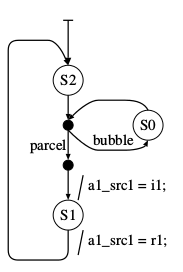
\includegraphics[height=20mm]{figs/something.png}
  \caption{This is the caption}
  \label{fig:something}
\end{figure}

\subsection{Tables}

A table is shown in \cref{tab:table-info}:

\begin{table}[h]
  \centering
  \begin{tabular}{cl|r}
    \multicolumn{3}{c}{\textbf{STUDENT INFORMATION}} \\
    \toprule
    First Name  & Last Name & Age \\
    \midrule
    John & Smith & 21\\
    Jack & Hoggs & 23\\
    Joey & Admin & 22\\
    \bottomrule
  \end{tabular}
  \caption{This is a table with good information}
  \label{tab:table-info}
\end{table}


\subsection{Lists}
\subsubsection{Numbered}
\begin{enumerate}
  \item First entry
  \item Second entry
  \item Third Entry
\end{enumerate}

\subsubsection{Descriptive}
\begin{description}
  \item[Reason 1]Because this is cool
  \item[Reason 2]Beacuse $2+2=4$
\end{description}

\subsubsection{Simple List}
\begin{list}{+}{}
\item Joe
\item Jack
\item \verb#Hello world!#
\item Hey
\end{list}

\subsection{Code and Pre-formatted Text}
This code will print \verb!Hello world! in Scala:
\begin{verbatim}
def main(args: Array[String]) = {
  println("Hello world!")
}
\end{verbatim}

\chapter{More math practice}

\section{Greek letters}
Various Greek letters are presented in \cref{tab:greek-letters}

\begin{table}[h]
  \centering
  \begin{tabular}{lc}
    \toprule
    Command           & Symbol \\
    \midrule
    \verb!\Delta!     & $\Delta$ \\
    \verb!\delta!     & $\delta$ \\
    \verb!\epsilon!   & $\epsilon$ \\
    \verb!\phi!       & $\phi$ \\
    \verb!\pi!        & $\pi$ \\
    \verb!\Pi!        & $\Pi$ \\
    \verb!\bar a!     & $\bar a$ \\
    \bottomrule
  \end{tabular}
  \caption{Greek letters and their corresponding command}
  \label{tab:greek-letters}
\end{table}

\section{More complicated mathematical description}
\subsection{Describing a set}
A random set $A$ is described using \verb!\begin{cases}...\end{cases}! in \cref{eq:set-desc} using a large font:
\begin{equation}
  \large
  x \in A \leftrightarrow \begin{cases}
    x/2 \leq 16     &\mbox{if } x > 4 \\
    3 < x^2 \leq 16 &\mbox{when } x \leq 4 \\
  \end{cases}
  \label{eq:set-desc}
\end{equation}


After the equation is done, the font becomes a normal size again. So this is how life
goes you know buddy I can't do anything but write garbage text---or should I?

\subsection{Integrals}

Integrals are written as described in \cref{eq:integral-eq}:
\begin{equation}
  \int_{-\pi}^{\infty}xdx
  \label{eq:integral-eq}
\end{equation}
